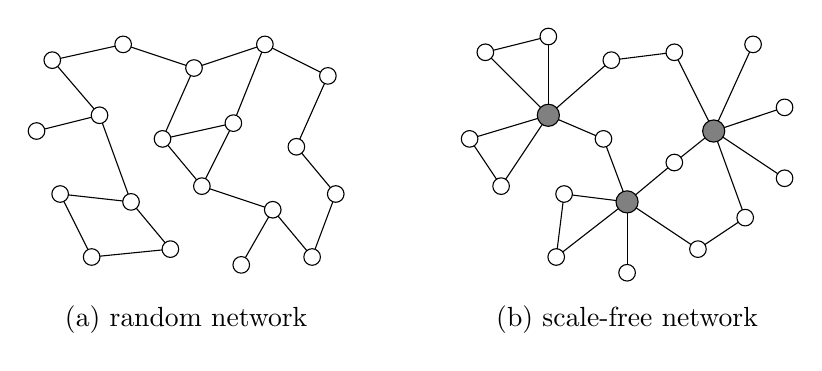
\begin{tikzpicture}[
  v/.style={circle, draw, fill=white, minimum size=6pt, inner sep=0pt},
  hub/.style={circle, draw, fill=gray, minimum size=8pt, inner sep=0pt}]
% (a) random network: degrees all small and similar
\begin{scope}
  \foreach \n/\x/\y in {1/0.3/2.6,2/1.2/2.8,3/2.1/2.5,4/3.0/2.8,5/3.8/2.4,
    6/0.1/1.7,7/0.9/1.9,8/1.7/1.6,9/2.6/1.8,10/3.4/1.5,
    11/0.4/0.9,12/1.3/0.8,13/2.2/1.0,14/3.1/0.7,15/3.9/0.9,
    16/0.8/0.1,17/1.8/0.2,18/2.7/0.0,19/3.6/0.1}
    \coordinate (r\n) at (\x,\y);
  \foreach \s/\t in {1/2,1/7,2/3,3/8,3/4,4/5,5/10,6/7,7/12,8/13,9/4,9/13,
    10/15,11/12,11/16,12/17,13/14,14/18,15/19,16/17,8/9,19/14}
    \draw (r\s) -- (r\t);
  \foreach \n in {1,...,19} \node[v] at (r\n) {};
  \node at (2,-0.7) {(a) random network};
\end{scope}
% (b) scale-free network: a few hubs with many links
\begin{scope}[xshift=5.6cm]
  \coordinate (H1) at (1.0,1.9); \coordinate (H2) at (2.0,0.8); \coordinate (H3) at (3.1,1.7);
  \foreach \n/\x/\y in {a/0.2/2.7,b/1.0/2.9,c/0.0/1.6,d/1.8/2.6,e/0.4/1.0,
    p/1.7/1.6,f/1.1/0.1,g/2.0/-0.1,h/2.9/0.2,q/1.2/0.9,
    j/2.6/2.7,k/3.6/2.8,l/4.0/2.0,m/4.0/1.1,n/3.5/0.6,o/2.6/1.3}
    \coordinate (\n) at (\x,\y);
  \foreach \z in {a,b,c,d,e,p} \draw (H1) -- (\z);
  \foreach \z in {f,g,h,q,p,o} \draw (H2) -- (\z);
  \foreach \z in {j,k,l,m,n,o} \draw (H3) -- (\z);
  \foreach \s/\t in {a/b,d/j,h/n,c/e,f/q}
    \draw (\s) -- (\t);
  \foreach \n in {a,b,c,d,e,p,f,g,h,q,j,k,l,m,n,o} \node[v] at (\n) {};
  \foreach \n in {H1,H2,H3} \node[hub] at (\n) {};
  \node at (2,-0.7) {(b) scale-free network};
\end{scope}
\end{tikzpicture}
